\newpage
\subsection{Application to Optimisation}
\begin{figure}[ht]
    \centering
    \begin{subfigure}[b]{0.45\textwidth}
        \centering
        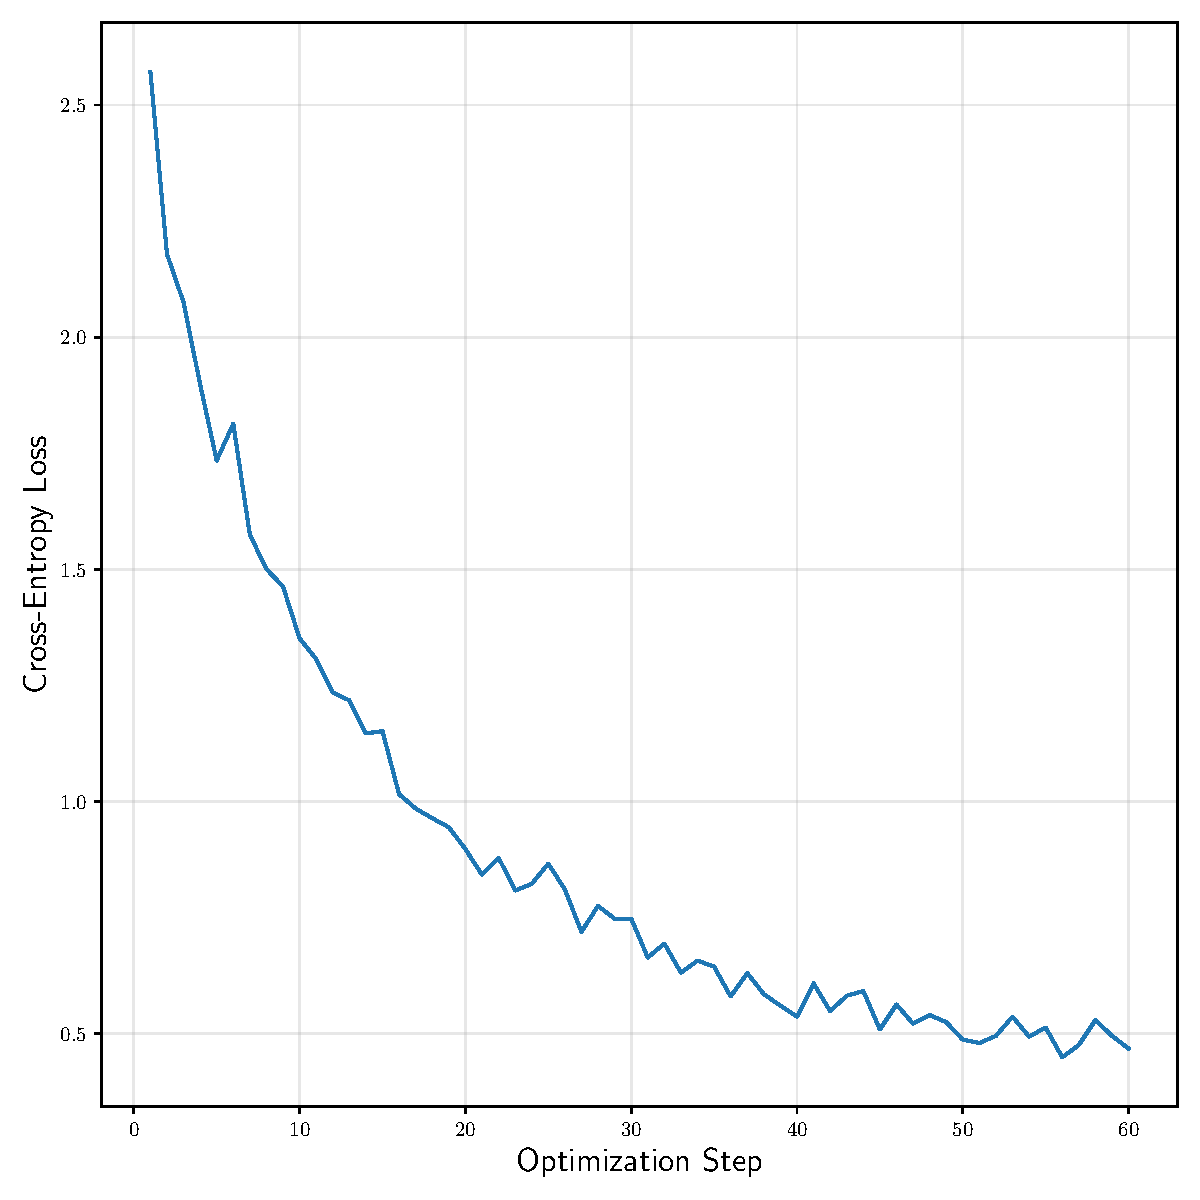
\includegraphics[width=0.8\linewidth]{../plots/mnist_loss.pdf}
        \caption{MNIST objective function}
        \label{fig:mnist-loss}
    \end{subfigure}
    \hfill
    \begin{subfigure}[b]{0.45\textwidth}
        \centering
        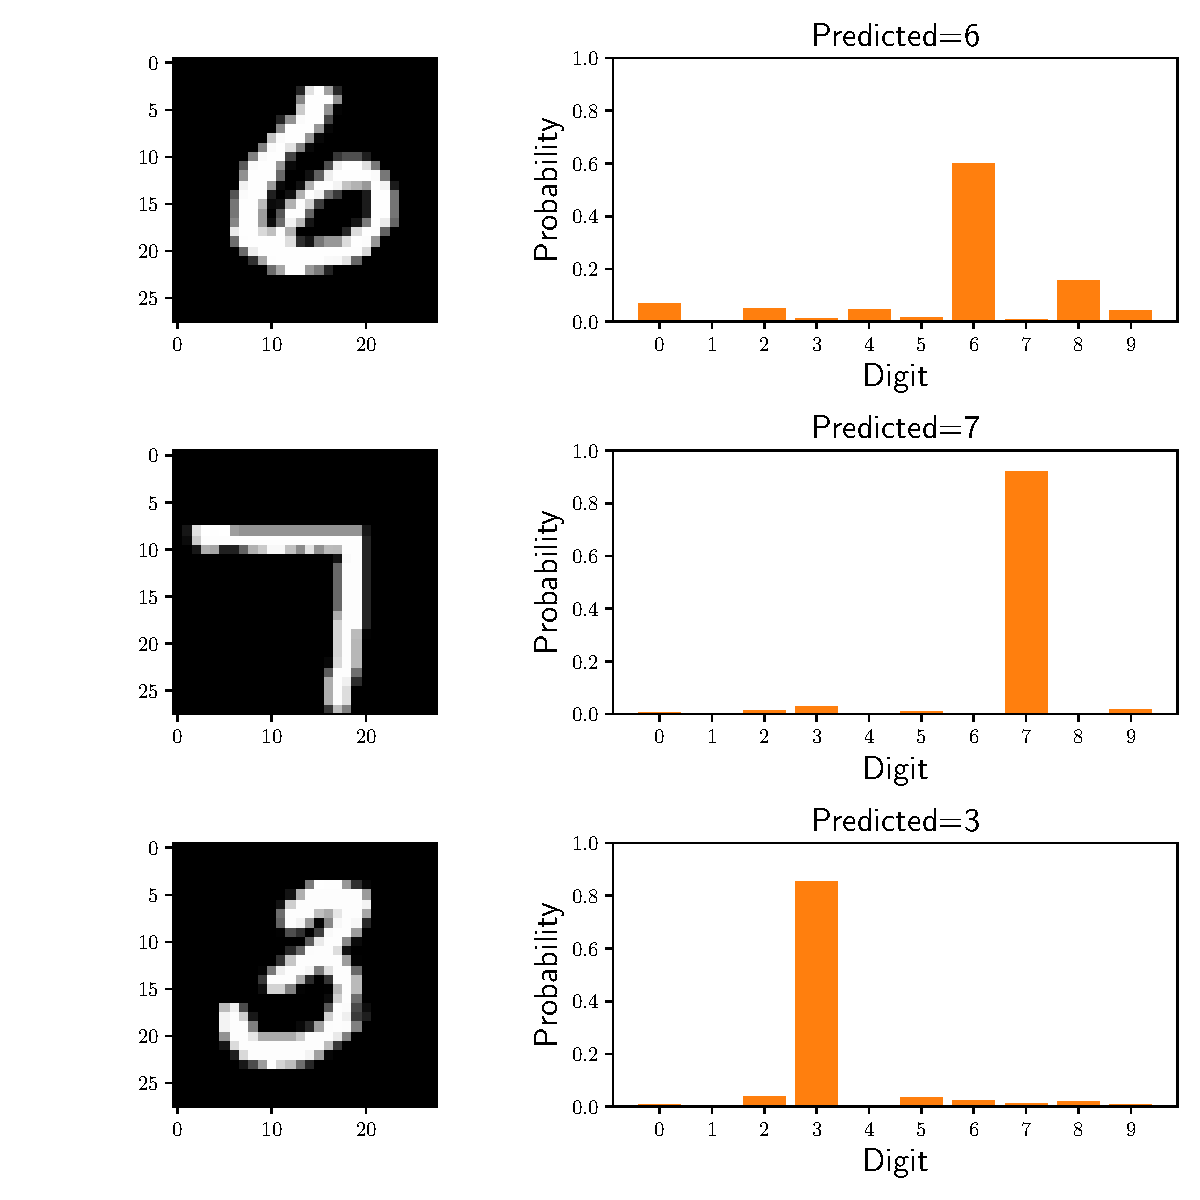
\includegraphics[width=0.8\linewidth]{../plots/mnist_predictions.pdf}
        \caption{MNIST images and pred. digit distr.}
        \label{fig:mnist-predictions}
    \end{subfigure}
\end{figure}

\begin{definition}[Cross-Entropy]
    Let $p, q$ be probability mass functions over the set $\mathcal{X}$
    and $X \sim p$.
    Then Cross-Entropy is defined as
    \[
        \CrossEntropy(p, q) = H(X) + D(p \| q)
    \]
\end{definition}

\begin{theorem} \label{theorem:cross-entropy-properties}
    \begin{enumerate}
        \item
            \[
                \min_{q}{\CrossEntropy(p, q)} = \min_{q}{D(p \| q)}
            \]
        \item
            \[
                \CrossEntropy(p, q) = -\sum_{x \in \mathcal{X}}{p(x) \log q(x)}
            \]
    \end{enumerate}
\end{theorem}
\begin{proof}
    \begin{enumerate}
        \item Cross-Entropy is simply Relative Entropy with a constant offset. So minimizing with respect to $q$ yields the same value.
        \item
            Let $X \sim p$. Then we have
            \begin{align*}
                \CrossEntropy(p, q) &= H(X) + D(p \| q)
                = \sum_{x \in \mathcal{X}}{-p(x) \log p(x)} + \sum_{x \in \mathcal{X}}{p(x) \log\frac{p(x)}{q(x)}} \\
                &= \sum_{x \in \mathcal{X}}{-p(x) \log p(x) + p(x) \log p(x) - p(x) \log q(x)} \\
                &= -\sum_{x \in \mathcal{X}}{p(x) \log q(x)}
            \end{align*}
    \end{enumerate}
\end{proof}

\begin{example}[MNIST Digit Classification]
    We can now apply the concept of Relative Entropy to solve a common classification problem from machine learning.
    Let $\Omega$ be the set of $28$x$28$ pixel images that contain exactly one handwritten digit from $0$ to $9$.
    The task is to predict the digit $0$ to $9$, based on the input image $\omega \in \Omega$. \\
    In order to accomplish this task, we define a model $f: \mathbb{R}^n \rightarrow \mathbb{R}_{+}^{10}$ with $n \in \mathbb{N}$. \\
    This function $f$ takes parameters as inputs that allow it to output a probability mass function that indicates the digit in the image.
    So $\forall \omega \in \Omega\vcentcolon f(\omega) \ge 0 \land \sum_{i=1}^{10} f(\omega)_i = 1$. \\
    The optimisation objective is
    \[
        \Phi = \argmin_{\phi \in \mathbb{R}^n}{D(d \| f_{\phi})}
    \]
    which according to Theorem \ref{theorem:cross-entropy-properties} is equivalent to
    \[
        \Phi = \argmin_{\phi \in \mathbb{R}^n}{\CrossEntropy(d, f_{\phi})}
    \]
    As we have shown in Theorem \ref{theorem:convexity-of-entropy}, the Relative Entropy and Cross-Entropy are convex functions. \\
    For $f$, we can use a two-layer convolutional neural network with dropout, as detailed in the official PyTorch Python example \cite{Pytorch:MNIST}.
    The solver is Tinygrad \cite{Tinygrad}.
    In this case, the model $f$ is not a convex function itself. So the optimisation objective is not convex either.
    But at least the loss function $\CrossEntropy(d \| .)$ is convex.
    We can now use Stochastic Gradient Descent to optimise for $60$ steps with step size 5e-3 and batch size $512$.
    Figure \ref{fig:mnist-loss} illustrates the Value of the Objective Function over time 
    and Figure \ref{fig:mnist-predictions} illustrates the outputs of the finished model.
\end{example}
